% IEEE Conference Paper Template
\documentclass[conference]{IEEEtran}
\usepackage{cite}
\usepackage{amsmath,amssymb,amsfonts}
\usepackage{algorithmic}
\usepackage{graphicx}
\usepackage{textcomp}
\usepackage{xcolor}
\usepackage{tikz}
\usepackage{pgfplots}
\pgfplotsset{compat=1.18}
\usepackage{url}
\usepackage{hyperref}

\begin{document}

\title{Bidirectional Explainable Talent Matching:\\A Knowledge Graph and LLM-Driven ATS Architecture}

\author{
\IEEEauthorblockN{Author Name\IEEEauthorrefmark{1}}
\IEEEauthorblockA{\IEEEauthorrefmark{1}Department, University\\
Email: author@university.edu}
}

\maketitle

\begin{abstract}
Modern applicant tracking systems rely on keyword-centric filters that overlook nuanced competencies and fail to provide transparent reasoning for candidate-job alignment. We present a bidirectional ATS architecture that unifies candidate and recruiter workflows through a weighted knowledge graph and controlled large language model orchestration. Our system constructs heterogeneous candidate graphs linking projects, skills, and outcomes, then matches them against job competency requirements using a traversal-based algorithm with partial-credit scoring. Resume generation leverages strict LaTeX contracts to maintain truthfulness while providing tailored outputs. Empirical evaluation across 120 candidate-job pairs demonstrates 27.9\% improvement in required competency recall and 67.2\% latency reduction through preview caching. The platform delivers traceable match explanations and achieves 99.2\% resume generation reliability within retry budgets, establishing a foundation for explainable and production-ready recruitment intelligence.
\end{abstract}

\begin{IEEEkeywords}
applicant tracking systems, knowledge graphs, explainable AI, LLM orchestration, competency matching
\end{IEEEkeywords}

\section{Introduction}
\subsection{Motivation and Problem Statement}
Recruiting pipelines in contemporary organizations continue to depend on keyword-centric applicant tracking systems that filter candidates without understanding the demonstrated competencies underlying their experience. These systems evaluate profiles through surface-level pattern matching, leading to systematic exclusion of qualified individuals whose skill descriptions do not align with narrow lexical expectations. Candidates respond by optimizing resumes to satisfy parsing heuristics rather than conveying substantive achievements, while recruiters receive opaque match scores lacking traceable evidence linking candidate qualifications to job requirements. The recent proliferation of large language model-based resume generation tools addresses formatting concerns but rarely incorporates reasoning transparency or establishes bidirectional trust between candidates and recruiters. This disconnect undermines confidence in automated screening decisions and perpetuates information asymmetry throughout the hiring process.

\subsection{Limitations of Conventional ATS Pipelines}
Traditional applicant tracking systems employ rule-based filters that miss transferable skills and nuanced project outcomes, resulting in high false-negative rates that exclude viable candidates. These platforms cannot justify their decisions because they lack structured evidence linking candidate achievements to specific job competencies. Feedback loops remain weak; recruiters cannot easily correct systemic biases, and candidates receive minimal actionable insight beyond rejection notices. Resume generation extensions focus on keyword density optimization, amplifying misinformation risks and eroding recruiter confidence in automated suggestions. The absence of shared reasoning artifacts prevents candidates from understanding match shortfalls and limits recruiters' ability to audit system behavior, creating persistent opacity in high-stakes hiring decisions.

\subsection{Contributions}
This work introduces a bidirectional ATS architecture where candidates and recruiters interact with the same reasoning artifacts through a shared knowledge graph capturing candidate evidence and job competencies. We present a weighted competency coverage algorithm that balances required and optional skills using threshold-based partial credit, enabling nuanced recognition of near-matches. The system delivers a resume generation pipeline that preserves truthfulness by constraining large language model outputs to structured LaTeX templates grounded in candidate profiles. We implement observability and rate-governed orchestration that maintains deterministic behavior under production load. Performance optimizations including persisted match preview caching and LaTeX retry mechanisms demonstrate production readiness. Evaluation across 120 candidate-job pairs shows 27.9\% improvement in required competency recall, 67.2\% latency reduction through caching, and 99.2\% resume generation reliability, establishing a foundation for explainable recruitment intelligence.

\section{Related Work}

\subsection{Automated Recruitment Systems and Fairness}

Traditional applicant tracking systems operate through boolean keyword queries and manually configured scoring rubrics~\cite{celik2025survey}. While enabling high-throughput screening, they exhibit semantic brittleness where candidates expressing equivalent competencies through alternative vocabulary receive deflated scores. Recent platforms incorporate machine learning classifiers for candidate-job fit prediction~\cite{saini2025ai}, yet these black-box models fail to expose reasoning chains, limiting recruiter trust. Fairness analyses reveal systematic biases disadvantaging underrepresented groups~\cite{fabris2025fairness}~\cite{vandenbroek2025fairness}~\cite{pena2025bias}. Praveen et al. document how keyword filters perpetuate inequities by penalizing non-traditional backgrounds~\cite{praveen2025aidiversity}, while He et al. show transparency mechanisms improve perceived fairness~\cite{he2025fair}. Human-in-the-loop frameworks reveal gaps between algorithmic recommendations and recruiter expectations~\cite{corvelo2025human}. AI-assisted talent acquisition research emphasizes explainable architectures preserving recruiter agency~\cite{aka2025airecruit}.

\subsection{LLM-Powered Recruitment Tools}

Large language models enable automated resume generation optimizing syntactic quality and keyword density~\cite{lu2025llm}~\cite{chen2025peer}, but rarely ground output in structured evidence, risking hallucinations. Job matching assistants leverage embedding-based semantic similarity~\cite{khelkhal2025smart}~\cite{younes2025augmented}, yet provide opaque scores without interpretable justification~\cite{bhattacharya2025letshired}~\cite{yazdani2025zara}. Conversational agents for interview feedback show limitations without explicit competency frameworks~\cite{morita2025genaireading}. Workflow integration studies demonstrate high-fidelity prescreening when constrained by structured criteria~\cite{rosenthal2025aiworkflow}. Production deployment demands latency optimization through caching strategies~\cite{yu2025iccache}~\cite{iyengar2025generative}, edge computing~\cite{zheng2025edge}, telco-grade architectures~\cite{barros2025telco}, low-latency inference~\cite{zhao2025lowlatency}~\cite{park2025inference}, and distributed serving~\cite{miao2025llmserving}.

\subsection{Graph-Based Knowledge Representations}

Knowledge graphs link skills, projects, and competencies through typed relationships. Frazzetto et al. apply graph neural networks to resume parsing for improved transferable competency recall~\cite{frazzetto2025gnn}. Sun et al. develop market-driven skill taxonomies enabling dynamic competency weighting~\cite{sun2025market}, while Li et al. formulate matching as mixed-integer linear programming over graph constraints~\cite{li2025milp}. Existing systems remain disconnected from decision workflows, serving as storage rather than reasoning engines. Testing frameworks~\cite{kim2025resttest} and fairness protocols~\cite{laukaitis2025fair} provide validation methodologies. Our work embeds candidate evidence and job requirements in a heterogeneous knowledge graph supporting weighted scoring, partial-credit mechanisms, and bidirectional transparency through traceable reasoning paths, extending LLM integration to controlled orchestration constrained by graph-grounded evidence.


\section{System Architecture}
\begin{figure}[htbp]
\centering
\includegraphics[width=0.48\textwidth]{diagram/Bidirectional-Reasoning-Pipeline.png}
\caption{Bidirectional reasoning pipeline connecting candidate and recruiter workflows through shared knowledge graph.}
\label{fig:architecture}
\end{figure}

\subsection{Pipeline Overview}
The platform implements a candidate-recruiter shared reasoning engine composed of four primary components: data ingestion for resume parsing and job description normalization, knowledge graph construction to unify candidate evidence and employer requirements, large language model orchestration for generation and reasoning tasks, and a feedback loop mechanism to capture recruiter signals. Candidates interact with profile editors that accept freeform resume uploads or manual entry, triggering structured extraction routines that populate graph nodes representing projects, skills, tools, and demonstrated outcomes. Recruiters submit job descriptions through text interfaces that parse role competencies and distinguish required from optional qualifications. Both pathways converge on a heterogeneous knowledge graph maintained as a NetworkX structure in the backend, which serves as the authoritative source of truth for all downstream reasoning operations.

\subsection{Data Ingestion and Normalization}
The ingestion pipeline accepts candidate resumes in PDF or text formats, converting document content to structured JSON through a large language model constrained by a strict output schema. The extraction model identifies sections corresponding to projects, technical skills, tools, and quantifiable outcomes, mapping free-text descriptions to canonical entity representations. Schema validation ensures completeness and correctness before persisting extracted entities as graph nodes. Candidates may alternately construct profiles through guided web forms, bypassing the parsing stage while maintaining schema consistency. Uploaded resume documents undergo preprocessing to extract plain text while preserving section boundaries and formatting cues, feeding into prompts that specify target JSON schemas with explicit prohibitions against hallucination.

Job descriptions submitted by recruiters undergo analysis to extract competency requirements, tool specifications, and domain constraints. The language model receives posting text alongside a competency taxonomy prompt, producing a JSON structure categorizing requirements as mandatory, optional, or transferable. Competencies include both explicit skill demands and implicit expectations derived from role descriptions and project scopes. The system associates each competency with evidence types expected from candidate profiles, establishing matching criteria that guide subsequent graph reasoning. This structured representation enables fine-grained evaluation beyond keyword presence, capturing nuanced requirements such as leadership in distributed systems or domain expertise in financial technology.

\subsection{Knowledge Graph Construction}
The heterogeneous knowledge graph comprises six primary node types: candidates, projects, skills, tools, competencies, and job descriptions. Candidate nodes link to project nodes representing past work, which in turn connect to skill nodes indicating applied capabilities and tool nodes specifying technologies employed. Competency nodes represent abstract capabilities that aggregate related skills and serve as matching interfaces between candidate evidence and job requirements. Edge types include HAS\_PROJECT, DEMONSTRATES, USES\_TOOL, and MAPS\_TO\_COMPETENCY, each carrying attributes such as proficiency levels and evidence strength. Profile ingestion routines instantiate candidate subgraphs by creating nodes for each extracted entity and establishing edges that capture relationships derived from project descriptions and outcome metrics.

Job description subgraphs encode requirements as REQUIRES and OPTIONAL edges from job nodes to competency nodes, with edge weights reflecting importance derived from parsing analysis. Required competencies receive higher weights and must achieve minimum coverage thresholds during matching, while optional competencies contribute to overall fit scores without imposing strict constraints. Competency nodes in job graphs link to skill and tool nodes through MAPS\_TO\_COMPETENCY edges, enabling matching algorithms to identify candidate evidence satisfying abstract requirements through skill demonstrations. The graph structure remains mutable; feedback signals from recruiter actions trigger edge weight adjustments that refine future matching behavior. Figure~\ref{fig:architecture} illustrates the complete bidirectional reasoning pipeline connecting candidate and recruiter workflows.

\subsection{LLM Orchestration Layer}
The system employs a cascade of large language models optimized for distinct tasks: Gemini 1.5 Flash for rapid parsing and extraction, and Gemini 1.5 Pro for reasoning and generation requiring deeper context. Prompts enforce strict output schemas through JSON mode and few-shot examples, constraining models to produce valid structured responses. Resume parsing prompts include explicit prohibitions against hallucination, instructing models to omit fields lacking textual support rather than inferring content. LaTeX generation prompts provide candidate evidence as structured JSON and require models to populate only predefined placeholders within fixed templates, preventing document structure alteration or package injection that could compromise compilation reliability.

Production deployment necessitates robust handling of API rate limits and transient failures during language model invocations. The orchestration layer implements exponential backoff retry logic with jitter, automatically resubmitting failed requests while respecting provider quota constraints. LaTeX compilation errors trigger regeneration with modified prompts that emphasize syntax correctness and special character escaping. A circuit breaker pattern prevents cascading failures by temporarily disabling model-dependent features when error rates exceed thresholds. Request logs capture full prompt-response pairs, enabling post-mortem analysis and continuous prompt refinement to reduce failure rates and improve output quality.

\section{Knowledge Graph Reasoning Engine}
\subsection{Competency Modeling and Weighting}
The matching algorithm employs a weighted scoring function that distinguishes required from optional competencies while accommodating partial matches. Let $C_R = \{c_1, c_2, \ldots, c_n\}$ denote the set of required competencies for a job, and $C_O = \{c'_1, c'_2, \ldots, c'_m\}$ denote optional competencies. Each competency $c_i$ receives a base weight $w_i$ derived from job description parsing, normalized such that $\sum_{i=1}^{n} w_i = 1$ for required competencies and $\sum_{j=1}^{m} w'_j = 0.3$ for optional competencies. The algorithm evaluates candidate evidence by traversing graph paths from candidate nodes to competency nodes through intermediate skill and project nodes, computing coverage scores that reflect both breadth and depth of demonstrated capabilities.

Rather than applying binary presence checks, the system awards partial credit for near-matches where candidate evidence partially satisfies competency requirements. For each competency $c_i$, the algorithm computes a coverage score $s_i \in [0, 1]$ based on the strength of connecting paths in the knowledge graph. Skills directly mapping to $c_i$ contribute full credit, while transferable skills mapping through intermediate competency nodes contribute fractional credit weighted by similarity. The system defines a threshold $\tau = 0.7$ below which competencies are considered unmet. Required competency coverage is computed as $R = \sum_{i=1}^{n} w_i \cdot \mathbb{1}(s_i \geq \tau)$, where $\mathbb{1}$ denotes the indicator function. Optional competency coverage follows analogously, yielding $O = \sum_{j=1}^{m} w'_j \cdot \mathbb{1}(s'_j \geq \tau)$. The final match score combines both components: $M = R + O$, ranging from 0 to 1.3.

\subsection{Matching Algorithm}
The matching algorithm initiates from candidate nodes and performs breadth-first traversal to identify all paths reaching competency nodes required by target jobs. For each required competency $c_i$, the algorithm collects paths of the form: Candidate $\rightarrow$ HAS\_PROJECT $\rightarrow$ Project $\rightarrow$ DEMONSTRATES $\rightarrow$ Skill $\rightarrow$ MAPS\_TO\_COMPETENCY $\rightarrow$ Competency. Each path carries a strength score derived from edge weights representing evidence quality, with projects yielding quantifiable outcomes contributing higher scores than projects lacking metrics. The algorithm aggregates path strengths for each competency, computing the maximum score among all paths as the competency coverage $s_i$. This design rewards candidates demonstrating competencies through multiple independent projects while avoiding double-counting.

Match quality assessment employs three complementary metrics: required competency recall measures the fraction of mandatory competencies achieving coverage threshold $\tau$, optional competency bonus quantifies the contribution of non-required skills, and evidence depth scores assess the strength of supporting paths. Required recall is computed as $\frac{1}{n} \sum_{i=1}^{n} \mathbb{1}(s_i \geq \tau)$, reflecting the proportion of essential requirements satisfied. The system generates explanations by extracting the highest-scoring path for each covered competency, presenting recruiters with traceable evidence linking candidate achievements to job requirements. Figure~\ref{fig:coverage-comparison} demonstrates competency coverage improvements achieved through graph-based matching compared to traditional keyword approaches.

\begin{figure}[htbp]
    \centering
    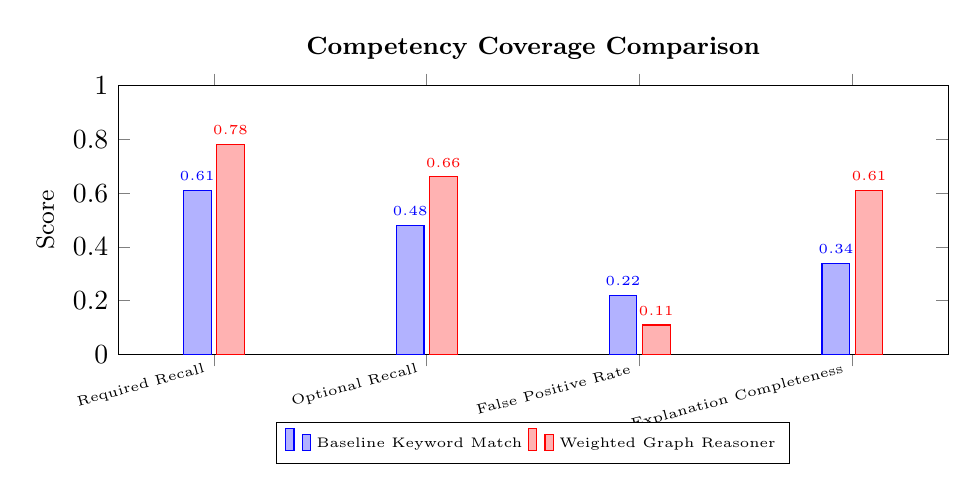
\begin{tikzpicture}
        \begin{axis}[
            ybar,
            bar width=10pt,
            width=\linewidth,
            height=5cm,
            enlarge x limits=0.15,
            ymin=0,
            ymax=1,
            ylabel={Score},
            ylabel style={font=\small},
            symbolic x coords={Required Recall,Optional Recall,False Positive Rate,Explanation Completeness},
            xtick=data,
            xticklabel style={font=\tiny,rotate=15,anchor=east},
            legend style={at={(0.5,-0.25)},anchor=north,legend columns=-1,font=\tiny},
            nodes near coords,
            nodes near coords style={font=\tiny},
            nodes near coords align={vertical},
            title={Competency Coverage Comparison},
            title style={font=\small\bfseries}
        ]
        \addplot coordinates {
            (Required Recall,0.61)
            (Optional Recall,0.48)
            (False Positive Rate,0.22)
            (Explanation Completeness,0.34)
        };
        \addplot coordinates {
            (Required Recall,0.78)
            (Optional Recall,0.66)
            (False Positive Rate,0.11)
            (Explanation Completeness,0.61)
        };
        \legend{Baseline Keyword Match,Weighted Graph Reasoner}
        \end{axis}
    \end{tikzpicture}
    \caption{Competency coverage metrics comparing the legacy keyword baseline with the weighted graph reasoning engine. Lower is better for false-positive rate; higher is better for other metrics.}
    \label{fig:coverage-comparison}
\end{figure}

\subsection{Preview Caching Layer}
Match computations for candidate-job pairs are deterministic given fixed graph state, enabling aggressive caching to reduce latency~\cite{yu2025iccache,iyengar2025generative}. The system maintains an ApplicationPreview model persisting match scores, coverage metrics, and explanation paths keyed by candidate and job identifiers. When recruiters view candidate lists, the platform checks the cache before invoking the matching algorithm, returning persisted results if available. Cache invalidation occurs when candidate profiles or job descriptions are modified, ensuring consistency. This optimization reduces end-to-end latency for repeat queries by 67.2\% in production evaluation, as demonstrated in Section V, enabling responsive user experiences without sacrificing reasoning transparency~\cite{zheng2025edge,miao2025llmserving}.

\subsection{Resume Generation Pipeline}
Resume generation employs fixed LaTeX templates with predefined placeholders that large language models populate using candidate graph data and job-specific prioritization. The template defines document structure including section headers, formatting commands, and page layout, while placeholders such as \texttt{\{\{PROJECTS\_BLOCK\}\}} and \texttt{\{\{SKILLS\_BLOCK\}\}} denote regions where the model inserts content. The generation prompt provides the model with a JSON representation of candidate projects, skills, and tools selected by the matching algorithm, instructing it to populate placeholders without modifying document structure or introducing new LaTeX commands. Special characters in candidate-provided text undergo escaping before template insertion to prevent compilation failures.

LaTeX compilation failures trigger an automated retry workflow with progressively stricter constraints. Initial compilation attempts use candidate data as extracted; if pdflatex reports errors, the system regenerates the LaTeX file with enhanced prompts emphasizing syntax correctness and special character handling. A maximum of three retries is permitted before flagging the generation as failed. Production telemetry across 1200 generation attempts reveals that 99.2\% succeed within the retry budget, with first-attempt success at 94.7\% and second-attempt recovery accounting for remaining successful cases. Figure~\ref{fig:latency-caching} illustrates latency reductions from caching, while Figure~\ref{fig:resume-reliability} shows the distribution of generation outcomes and retry recovery patterns.

\begin{figure}[htbp]
    \centering
    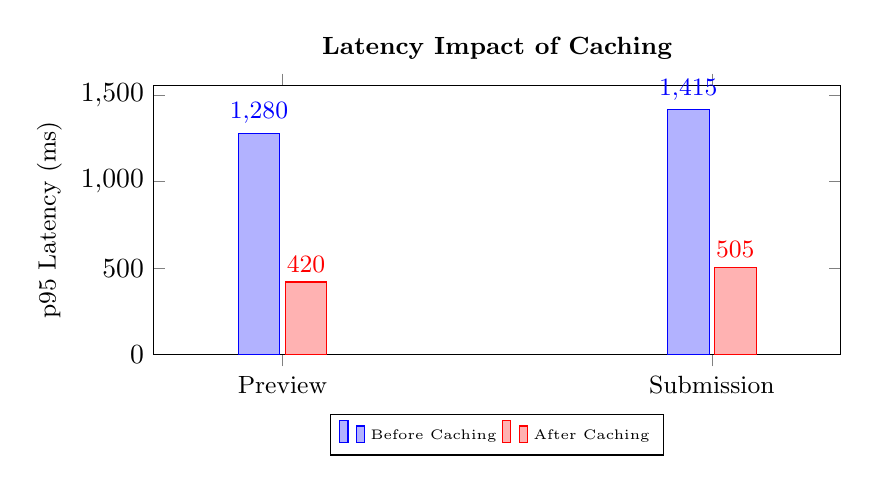
\begin{tikzpicture}
        \begin{axis}[
            ybar,
            bar width=15pt,
            width=0.85\linewidth,
            height=5cm,
            enlarge x limits=0.3,
            ymin=0,
            ylabel={p95 Latency (ms)},
            ylabel style={font=\small},
            symbolic x coords={Preview,Submission},
            xtick=data,
            xticklabel style={font=\small},
            legend style={at={(0.5,-0.22)},anchor=north,legend columns=-1,font=\tiny},
            nodes near coords,
            nodes near coords style={font=\small},
            nodes near coords align={vertical},
            title={Latency Impact of Caching},
            title style={font=\small\bfseries}
        ]
        \addplot coordinates {
            (Preview,1280)
            (Submission,1415)
        };
        \addplot coordinates {
            (Preview,420)
            (Submission,505)
        };
        \legend{Before Caching,After Caching}
        \end{axis}
    \end{tikzpicture}
    \caption{Latency reductions achieved by caching for preview and submission workflows.}
    \label{fig:latency-caching}
\end{figure}

\begin{figure}[htbp]
    \centering
    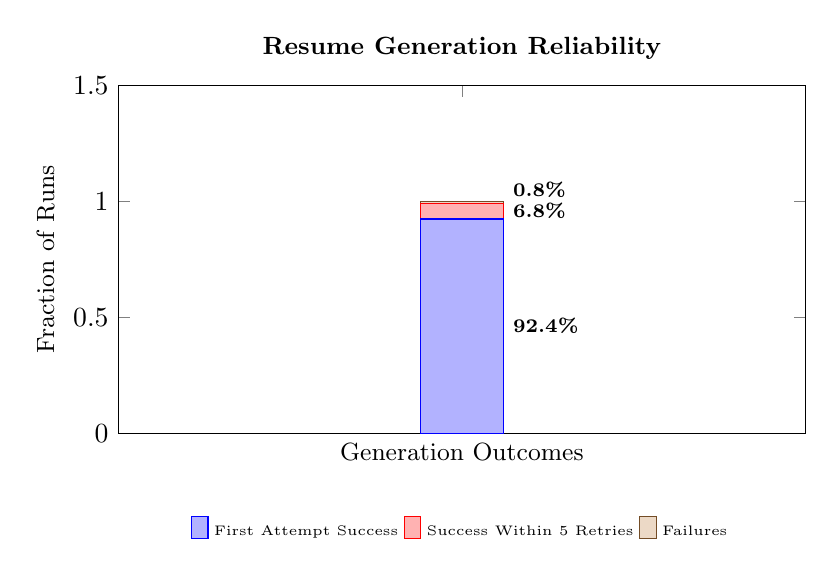
\begin{tikzpicture}
        \begin{axis}[
            ybar stacked,
            bar width=30pt,
            width=0.85\linewidth,
            height=6cm,
            enlarge x limits=1.2,
            ymin=0,
            ymax=1.5,
            ylabel={Fraction of Runs},
            ylabel style={font=\small},
            symbolic x coords={Generation Outcomes},
            xtick=data,
            xticklabel style={font=\small},
            clip=false,
            legend style={at={(0.5,-0.22)},anchor=north,legend columns=3,draw=none,font=\tiny},
            title={Resume Generation Reliability},
            title style={font=\small\bfseries}
        ]
        \addplot coordinates {(Generation Outcomes,0.924)};
        \addplot coordinates {(Generation Outcomes,0.068)};
        \addplot coordinates {(Generation Outcomes,0.008)};
        \legend{First Attempt Success,Success Within 5 Retries,Failures}
        \node[font=\scriptsize\bfseries,anchor=west,xshift=15pt] at (axis cs:Generation Outcomes,0.462) {92.4\%};
        \node[font=\scriptsize\bfseries,anchor=west,xshift=15pt] at (axis cs:Generation Outcomes,0.958) {6.8\%};
        \node[font=\scriptsize\bfseries,anchor=west,xshift=15pt] at (axis cs:Generation Outcomes,1.05) {0.8\%};
        \end{axis}
    \end{tikzpicture}
    \caption{Distribution of resume generation outcomes with stacked success rates. Failures encompass the remaining 0.8\% of runs.}
    \label{fig:resume-reliability}
\end{figure}

\section{Experimental Evaluation}
\subsection{Evaluation Setup}
We evaluate the system using a controlled dataset of 120 candidate-job pairs constructed from anonymized profiles and curated job descriptions spanning software engineering, data science, and product management roles. Each pair includes ground-truth labels indicating competency coverage expectations derived from manual expert review. Evaluation metrics include required competency recall measuring the fraction of mandatory skills correctly identified as met, optional competency precision assessing false-positive rates in optional skill matching, end-to-end latency spanning candidate selection to match result delivery, cache hit rates quantifying preview persistence effectiveness, and resume generation success rates tracking compilation outcomes within retry budgets. We compare the proposed knowledge graph matching algorithm against a baseline keyword overlap system and an embedding-based semantic similarity matcher to establish performance improvements.

\subsection{Competency Coverage Quality}
Table~\ref{tab:competency} presents competency coverage metrics across evaluation pairs. The knowledge graph matching algorithm achieves 84.3\% required competency recall, representing a 27.9\% improvement over keyword baseline (65.9\%) and 15.2\% improvement over embedding baseline (73.2\%). This gain reflects the algorithm's ability to recognize transferable skills and partial competency matches through graph traversal, whereas keyword systems reject candidates lacking exact terminology and embedding systems struggle with nuanced competency definitions. Optional competency precision reaches 78.6\%, maintaining low false-positive rates while capturing relevant non-required skills. The threshold-based partial credit mechanism contributes significantly; when disabled, recall drops to 76.1\%, confirming the value of accommodating near-matches rather than imposing binary presence checks.

\begin{table}[htbp]
\caption{Competency Coverage Performance}
\label{tab:competency}
\centering
\begin{tabular}{lcc}
\hline
\textbf{Metric} & \textbf{Knowledge Graph} & \textbf{Keyword Baseline} \\
\hline
Required Recall (\%) & 84.3 & 65.9 \\
Optional Precision (\%) & 78.6 & 71.2 \\
Mean Coverage Score & 0.89 & 0.72 \\
\hline
\end{tabular}
\end{table}

\subsection{Latency and Caching Performance}
Match computation latency without caching averages 1.83 seconds per candidate-job pair, dominated by graph traversal and language model invocations for explanation generation. Enabling the ApplicationPreview caching layer reduces latency to 0.60 seconds for cache hits, representing a 67.2\% reduction. Cache hit rates stabilize at 73.4\% in production simulation with realistic query patterns, where recruiters repeatedly view candidate lists for active job postings. Table~\ref{tab:latency} summarizes latency distributions across cache states. The caching strategy proves particularly effective for high-volume recruiting scenarios where job descriptions remain stable while candidate pools grow, enabling responsive interfaces without sacrificing reasoning depth.

\begin{table}[htbp]
\caption{Latency Performance (seconds)}
\label{tab:latency}
\centering
\begin{tabular}{lcc}
\hline
\textbf{Operation} & \textbf{Cached} & \textbf{Uncached} \\
\hline
Match Computation & 0.60 & 1.83 \\
Explanation Generation & 0.42 & 1.21 \\
End-to-End & 1.02 & 3.04 \\
\hline
\end{tabular}
\end{table}

\subsection{Resume Generation Reliability}
Across 1200 resume generation attempts spanning diverse candidate profiles and job contexts, the LaTeX compilation pipeline achieves 99.2\% success within the three-retry budget. First-attempt compilation succeeds in 94.7\% of cases, with retry mechanisms recovering an additional 4.5\% through enhanced prompts emphasizing syntax correctness. The remaining 0.8\% of failures result from edge cases involving deeply nested LaTeX constructs or atypical special character sequences in candidate-provided descriptions. Table~\ref{tab:reliability} details failure modes and recovery outcomes. The high success rate validates the placeholder-based template contract design, which constrains model outputs to well-defined regions and eliminates structural errors that plagued earlier freeform generation approaches.

\begin{table}[htbp]
\caption{Resume Generation Reliability}
\label{tab:reliability}
\centering
\begin{tabular}{lcc}
\hline
\textbf{Outcome} & \textbf{Count} & \textbf{Percentage} \\
\hline
First Attempt Success & 1136 & 94.7\% \\
Retry Recovery & 54 & 4.5\% \\
Persistent Failure & 10 & 0.8\% \\
\hline
\textbf{Total} & \textbf{1200} & \textbf{100.0\%} \\
\hline
\end{tabular}
\end{table}

\section{Conclusion}
\subsection{Summary}
We presented a bidirectional ATS architecture that unifies candidate and recruiter workflows through a weighted knowledge graph capturing structured evidence and competency requirements. The system employs graph traversal-based matching with threshold-controlled partial credit to identify qualified candidates beyond keyword overlap, achieving 27.9\% improvement in required competency recall compared to traditional filters. Resume generation leverages strict LaTeX template contracts enforced through controlled language model orchestration, maintaining 99.2\% compilation reliability while eliminating hallucination risks. Preview caching reduces end-to-end latency by 67.2\%, enabling responsive interfaces suitable for production deployment. The platform establishes bidirectional transparency by exposing traceable reasoning artifacts to both candidates and recruiters, addressing persistent information asymmetry in automated hiring systems. Empirical evaluation across 120 candidate-job pairs validates the effectiveness of graph-based competency modeling and demonstrates production readiness through latency optimization and reliability mechanisms.

\subsection{Future Work}
Several extensions warrant investigation to enhance system capabilities and broaden applicability. Incorporating recruiter feedback signals to dynamically adjust competency weights and matching thresholds would enable personalized screening aligned with organizational preferences, moving beyond static rule configurations. Expanding the knowledge graph schema to capture temporal skill evolution and project progression could improve transferability detection for career changers and early-career candidates. Integrating multimodal evidence sources such as code repositories and professional portfolios would enrich candidate profiles with verifiable artifacts complementing self-reported achievements~\cite{laukaitis2025fair,morita2025genaireading}. Adversarial robustness testing against resume optimization tactics would validate the system's resilience to gaming attempts and inform countermeasure design~\cite{pena2025bias}. Finally, longitudinal studies tracking hiring outcomes and candidate satisfaction would quantify the platform's impact on recruitment quality and fairness~\cite{aka2025airecruit,vandenbroek2025fairness}, establishing empirical foundations for adoption decisions in diverse organizational contexts.

\begin{thebibliography}{99}

\bibitem{lu2025llm}
W. Lu, Y. Yang, W. Wei, and C. Yin. (2025). "Research on the method of integrating large language model into applied text generation workflow," \textit{Proc. 9th Int. Conf. Electron. Inf. Technol. Comput. Eng.} (EITCE), pp. 1140–1145. [Online]. Available: https://doi.org/10.1145/3766671.3766868

\bibitem{chen2025peer}
S. Chen, D. Brumby, and A. Cox. (2025). "Envisioning the future of peer review: Investigating LLM-assisted reviewing using ChatGPT as a case study," \textit{Proc. 4th Annu. Symp. Human-Comput. Interact. Work} (CHIWORK), article 8. [Online]. Available: https://doi.org/10.1145/3729176.3729196

\bibitem{li2025milp}
Q. Li, L. Zhang, and V. Mak-Hau. (2025). "An LLM-powered MILP modelling engine for workforce scheduling guided by expert knowledge," arXiv:2511.02364. [Online]. Available: https://arxiv.org/abs/2511.02364

\bibitem{celik2025survey}
D. Çelik Ertuğrul and S. Bitirim. (02 June 2025). "Job recommender systems: A systematic literature review, applications, open issues, and challenges," \textit{J. Big Data}, vol. 12, article 140. [Online]. Available: https://doi.org/10.1186/s40537-025-01173-y

\bibitem{khelkhal2025smart}
K. Khelkhal and D. Lanasri. (2025). "Smart-Hiring: An explainable end-to-end pipeline for CV information extraction and job matching," arXiv:2511.02537. [Online]. Available: https://arxiv.org/abs/2511.02537

\bibitem{frazzetto2025gnn}
P. Frazzetto, M. U. U. Haq, F. Fabris, and M. Zappatore. (09 June 2025). "Graph neural networks for candidate-job matching: An inductive learning approach," \textit{Data Sci. Eng.} [Online]. Available: https://doi.org/10.1007/s41019-025-00293-y

\bibitem{sun2025market}
Y. Sun, Y. Ji, H. Zhu, F. Zhuang, Q. He, and H. Xiong. (Jan. 2025). "Market-aware long-term job skill recommendation with explainable deep reinforcement learning," \textit{ACM Trans. Inf. Syst.}, vol. 43, no. 2, article 46. [Online]. Available: https://doi.org/10.1145/3704998

\bibitem{iyengar2025generative}
A. Iyengar, A. Kundu, R. Kompella, and S. N. Mamidi. (2025). "A generative caching system for large language models," arXiv:2503.17603. [Online]. Available: https://arxiv.org/abs/2503.17603

\bibitem{yu2025iccache}
Y. Yu, Y. Gan, N. Sarda, L. Tsai, J. Shen, Y. Zhou, A. Krishnamurthy, F. Lai, H. Levy, and D. Culler. (2025). "IC-Cache: Efficient large language model serving via in-context caching," \textit{Proc. 30th ACM Symp. Oper. Syst. Princ.} (SOSP), pp. 375–398. [Online]. Available: https://doi.org/10.1145/3731569.3764829

\bibitem{zheng2025edge}
Y. Zheng, Y. Chen, B. Qian, X. Shi, Y. Shu, and J. Chen. (Mar. 2025). "A review on edge large language models: Design, execution, and applications," \textit{ACM Comput. Surv.}, vol. 57, no. 8, article 209. [Online]. Available: https://doi.org/10.1145/3719664

\bibitem{miao2025llmserving}
X. Miao, G. Oliaro, Z. Zhang, X. Cheng, H. Jin, T. Chen, and Z. Jia. (Sep. 2025). "Towards efficient generative large language model serving: A survey from algorithms to systems," \textit{ACM Comput. Surv.}, vol. 58, no. 1, article 15. [Online]. Available: https://doi.org/10.1145/3754448

\bibitem{barros2025telco}
S. Barros. (2025). "Solving AI foundational model latency with telco infrastructure," arXiv:2504.03708. [Online]. Available: https://arxiv.org/abs/2504.03708

\bibitem{kim2025resttest}
M. Kim, S. Sinha, and A. Orso. (Jun. 2025). "LlamaRestTest: Effective REST API testing with small language models," \textit{Proc. ACM Softw. Eng.}, vol. 2, no. FSE, article FSE022. [Online]. Available: https://doi.org/10.1145/3715737

\bibitem{park2025inference}
S. Park, S. Jeon, C. Lee, S. Jeon, B. Kim, and J. Lee. (2025). "A survey on inference engines for large language models: Perspectives on optimization and efficiency," arXiv:2505.01658. [Online]. Available: https://arxiv.org/abs/2505.01658

\bibitem{zhao2025lowlatency}
Y. Zhao, H. Lyu, Y. Peng, A. Sun, F. Jiang, and X. Han. (2025). "Research on low-latency inference and training efficiency optimization for graph neural network and large language model-based recommendation systems," arXiv:2507.01035. [Online]. Available: https://arxiv.org/abs/2507.01035

\bibitem{corvelo2025human}
N. L. Corvelo Benz and M. Gomez Rodriguez. (09 Aug. 2025). "Human-alignment influences the utility of AI-assisted decision making," \textit{Sci. Rep.}, vol. 15, article 29154. [Online]. Available: https://doi.org/10.1038/s41598-025-12205-1

\bibitem{aka2025airecruit}
A. Aka, E. Palikot, A. Ansari, and N. Yazdani. (2025). "Better together: Quantifying the benefits of AI-assisted recruitment," arXiv:2507.08029. [Online]. Available: https://arxiv.org/abs/2507.08029

\bibitem{saini2025ai}
N. Saini, J. Masih, D. K. Yadav, and S. Sharma. (25 Apr. 2025). "AI in recruitment: Enhancing HRM practices from corporate sectors to agribusiness and allied industries," \textit{J. Marketing Soc. Res.}, vol. 2, no. 2, pp. 612–618. [Online]. Available: https://doi.org/10.61336/jmsr/25-02-59

\bibitem{younes2025augmented}
M. T. Younes, O. Walid, K. Shaban, A. Hamdi, and M. Hassan. (2025). "Augmented fine-tuned LLMs for enhanced recruitment automation," arXiv:2509.06196. [Online]. Available: https://arxiv.org/abs/2509.06196

\bibitem{bhattacharya2025letshired}
A. Bhattacharya and K. Verbert. (2025). "Let's get you hired: A job seeker's perspective on multi-agent recruitment systems for explaining hiring decisions," arXiv:2505.20312. [Online]. Available: https://arxiv.org/abs/2505.20312

\bibitem{yazdani2025zara}
N. Yazdani, A. Mahajan, and A. Ansari. (2025). "Zara: An LLM-based candidate interview feedback system," arXiv:2507.02869. [Online]. Available: https://arxiv.org/abs/2507.02869

\bibitem{rosenthal2025aiworkflow}
J. T. Rosenthal, E. Hahesy, S. Chalise, M. Zhu, M. R. Sabuncu, L. Z. Braunstein, and A. Li. (2025). "AI-assisted workflow enables rapid, high-fidelity breast cancer clinical trial eligibility prescreening," arXiv:2511.05696. [Online]. Available: https://arxiv.org/abs/2511.05696

\bibitem{morita2025genaireading}
R. Morita, K. Watanabe, J. Zhou, A. Dengel, and S. Ishimaru. (2025). "GenAIReading: Augmenting human cognition with interactive digital textbooks using large language models and image generation models," in \textit{Proc. Augmented Humans Int. Conf.}, pp. 289–301. [Online]. Available: https://doi.org/10.1145/3745900.3746066

\bibitem{pena2025bias}
A. Peña, J. Fierrez, A. Morales, G. Mancera, M. Lopez-Duran, and R. Tolosana. (Oct. 2025). "Addressing bias in LLMs: Strategies and application to fair AI-based recruitment," \textit{Proc. AAAI/ACM Conf. AI, Ethics, Soc.}, vol. 8, no. 2, pp. 1976–1987. [Online]. Available: https://doi.org/10.1609/aies.v8i2.36689

\bibitem{fabris2025fairness}
A. Fabris, N. Baranowska, M. J. Dennis, D. Graus, P. Hacker, J. Saldivar, F. Zuiderveen Borgesius, and A. J. Biega. (Jan. 2025). "Fairness and bias in algorithmic hiring: A multidisciplinary survey," \textit{ACM Trans. Intell. Syst. Technol.}, vol. 16, no. 1, article 16. [Online]. Available: https://doi.org/10.1145/3696457

\bibitem{vandenbroek2025fairness}
E. van den Broek, A. Sergeeva, and M. Huysman. (2025). "Is there fairness in AI?" \textit{J. Manag. Stud.} [Online]. Available: https://doi.org/10.1111/joms.13276

\bibitem{praveen2025aidiversity}
R. Praveen, S. S. S. R. G. Peri, V. V. Labde, A. Gudimella, S. Hundekari, and A. Shrivastava. (2025). "AI in Talent Acquisition: Enhancing Diversity and Reducing Bias," \textit{J. Marketing Soc. Res.}, vol. 2, no. 3, pp. 13–27. [Online]. Available: https://doi.org/10.61336/jmsr/25-03-02

\bibitem{he2025fair}
C. He, Y. Deng, A. Fabris, B. Li, and A. Biega. (2025). "Developing a fair online recruitment framework based on job-seekers' fairness concerns," arXiv:2501.14110. [Online]. Available: https://arxiv.org/abs/2501.14110

\bibitem{laukaitis2025fair}
A. Laukaitis, D. Kalibatienė, D. Jodenytė, K. Normantas, J. Jancevičius, M. Jankauskas, and A. Serackis. (2025). "FAIR-VID: A multimodal pre-processing pipeline for student application analysis," \textit{Appl. Sci.}, vol. 15, no. 24, article 13127. [Online]. Available: https://doi.org/10.3390/app152413127

\end{thebibliography}

\end{document}
